\documentclass[a4paper, 10pt, twoside]{article}

\usepackage[top=1in, bottom=1in, left=1in, right=1in]{geometry}
\usepackage[utf8]{inputenc}
\usepackage[spanish, es-ucroman, es-noquoting]{babel}
\usepackage{setspace}
\usepackage{fancyhdr}
\usepackage{lastpage}
\usepackage{amsmath}
\usepackage{xcolor}
\usepackage{amsfonts}
\usepackage{amsthm}
\usepackage{verbatim}
\usepackage{fancyvrb}
\usepackage{graphicx}
\usepackage{float}
\usepackage{bytefield}
\usepackage{enumitem} % Provee macro \setlist
\usepackage{tabularx}
\usepackage{multirow}
\usepackage{hyperref}
\usepackage{xspace}
\usepackage{qtree}
\usepackage{listings}
\usepackage{pgfplots}
\usepackage{algpseudocode}
\usepackage[toc, page]{appendix}

\definecolor{light-gray}{HTML}{E6E6E6}

\lstset{ %
backgroundcolor=\color{light-gray},
breaklines=true,
keepspaces=true,
language=C
}

%%%%%%%%%% Constantes - Inicio %%%%%%%%%%
\newcommand{\titulo}{Trabajo Práctico Final}
\newcommand{\materia}{Organización del computador 2}
\newcommand{\integrantes}{Lautaro Petaccio}
\newcommand{\cuatrimestre}{2016}
%%%%%%%%%% Constantes - Fin %%%%%%%%%%


%%%%%%%%%% Configuración de Fancyhdr - Inicio %%%%%%%%%%
\pagestyle{fancy}
\thispagestyle{fancy}
\lhead{\titulo\ · \materia}
\rhead{\integrantes}
\renewcommand{\footrulewidth}{0.4pt}
\cfoot{\thepage /\pageref{LastPage}}

\fancypagestyle{caratula} {
   \fancyhf{}
   \cfoot{\thepage /\pageref{LastPage}}
   \renewcommand{\headrulewidth}{0pt}
   \renewcommand{\footrulewidth}{0pt}
}
%%%%%%%%%% Configuración de Fancyhdr - Fin %%%%%%%%%%


%%%%%%%%%% Miscelánea - Inicio %%%%%%%%%%
% Evita que el documento se estire verticalmente para ocupar el espacio vacío
% en cada página.
\raggedbottom

% Separación entre párrafos.
\setlength{\parskip}{0.5em}

% Separación entre elementos de listas.
\setlist{itemsep=0.5em}

%%%%%%%%%%%%%%%%%%%%%%%%%%%%%%%%%%%%%%%%%%%%%%%%%%%%%%%%%%%%%%%%%%%%%%%%%%%%%%%
%% Carátula                                                                  %%
%%%%%%%%%%%%%%%%%%%%%%%%%%%%%%%%%%%%%%%%%%%%%%%%%%%%%%%%%%%%%%%%%%%%%%%%%%%%%%%

\begin{document}

\thispagestyle{caratula}

\begin{center}


\includegraphics[height=2cm]{DC.png} 
\hfill

\includegraphics[height=2cm]{UBA.jpg} 

\vspace{2cm}

Departamento de Computación,\\
Facultad de Ciencias Exactas y Naturales,\\
Universidad de Buenos Aires

\vspace{4cm}

\begin{Huge}
\titulo
\end{Huge}

\vspace{0.5cm}

\begin{Large}
\materia
\end{Large}

\vspace{1cm}

\cuatrimestre

\vspace{4cm}

\begin{tabular}{|c|c|c|}
\hline
Apellido y Nombre & LU & E-mail\\
\hline
Petaccio, Lautaro José & 443/11 & lausuper@gmail.com\\
\hline
\end{tabular}

\end{center}

\newpage

\tableofcontents

\newpage


%%%%%%%%%%%%%%%%%%%%%%%%%%%%%%%%%%%%%%%%%%%%%%%%%%%%%%%%%%%%%%%%%%%%%%%%%%%%%%%
%% Introducción                                                              %%
%%%%%%%%%%%%%%%%%%%%%%%%%%%%%%%%%%%%%%%%%%%%%%%%%%%%%%%%%%%%%%%%%%%%%%%%%%%%%%%

\section{Introducción}

\subsection{¿Qué son los Bitcoins?}
Los Bitcoins conforman una de las muchas\footnote{\href{http://dogecoin.com/}{DogeCoin}, \href{https://litecoin.com/}{LiteCoin}, etc.} \textit{crypto currencies} o monedas criptográgificas que existen hoy en día.

Se las llama \textit{currencies} por la posibilidad de poder realizar transacciones de las mismas entre usuarios o \textit{wallets}, pudiendo establecerse como moneda en un intercambio comercial. Los dueños de las billeteras son anónimos brindando el anonimato por el cuál son también conocidas.

La cantidad de Bitcoins en una \textit{wallet} es el resultado de todas las transacciones con la misma. Para mantener seguridad en las transacciones, es necesario un mecanismo de validación y verificación de las mismas. Esta verificación y validación es realizada a través de algoritmos criptográficos, de donde las monedas sacan el nombre de \textit{crypto}. En el caso del Bitcoin, el algoritmo criptográfico es el de SHA256d o double SHA256, y consiste en una doble aplicación del algoritmo de hashing SHA256.

\subsection{Block Chain}
La arquitectura detrás de los Bitcoins está formada pour una red descentralizada, no existe un ente regulador de las transacciones o billeteras que se crean, los usuarios serán los responsables de verificar y validar los eventos que ocurren en la red.

Todos los usuarios conservan una copia de la \textit{Block Chain}, una base de datos pública que contiene la información de todas las transacciones realizadas en la red. La información se replica entre los usuarios que desde ahora actuarán como nodos y mantendrán la misma actualizada.

\begin{figure}[h]
\centering
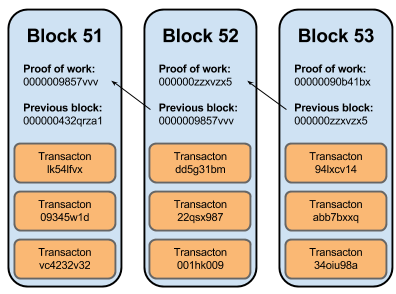
\includegraphics[height=6cm]{bitcoin-block-chain.png}
\caption{Ejemplo de la composición de la \textit{Block Chain}}
\end{figure}

La \textit{Block Chain} consiste en una serie de bloques encadenados. Cada bloque contiene el hash \footnote{El resultante de aplicar una función de hash criptográfica. En el caso de los Bitcoins, SHA256d} de una o más transacciones realizadas entre billeteras e información complementaria para validar el mismo:
\begin{itemize}
	\item \textbf{Height:} La altura en la cadena de bloques.
	\item \textbf{Block Reward:} La recompenza recibida por validar este bloque.
	\item \textbf{Timestamp:} El momento de la validación del bloque.
	\item \textbf{Merkle Root:} Es el hash, utilizando SHA256d de el hash de cada transacción.
	\item \textbf{Previous Block:} El bloque anterior en la cadena.
	\item \textbf{Difficulty:} La dificultad de validación del bloque que será utilizada por los \textit{miners}.
	\item \textbf{Next Block:} El próximo bloque en la cadena.
	\item \textbf{Nonce:} Un valor de 8 bytes en tamaño utilizado para la validación del bloque.
\end{itemize}

La Block Chain es pública, cada bloque puede ser accedido desde el sitio de blockexplorer \footnote{\href{http://testnet.blockexplorer.com}{Block Explorer}}, blockchain \footnote{\href{https://blockchain.info/}{Block Chain Info}} o cualquier otro de los disponibles.

\subsection{Generación de nuevos bloques y mining}
Minear Bitcoins es el término comúnmente referido al proceso de agregar nuevas transacciones válidas a la red mediante la generación de nuevos bloques que serán agregados a la \textit{Block chain}. Al agregarse el nuevo bloque, la red realizará una verificación basada en el trabajo realizado por el miner o trabajador, y agrega el bloque en caso de ser correcta. 

El trabajador que consigue que su bloque sea verificado por la red como correcto, recibe una cantidad de Bitcoins, convirtiendo al proceso de mining en la manera en la que se generan Bitcoins.

Al trabajo a realizar por los miners se lo llama \textit{proof of work} y tiene como objetivo ser un proceso computacionalmente complejo para los siguientes propósitos:
\begin{itemize}
	\item Mantener estable en el tiempo el descubrimiento de bloques y así, la generación de Bitcoins. Esto es posible de realizar mediante la variación de dificultad del trabajo.
	\item Como una manera de seguridad, para imposibilitar o mitigar ataques sobre la verificación de transacciones\footnote{https://en.bitcoin.it/wiki/Double-spending}.
\end{itemize}

Para la realización del \textit{proof of work}, se necesita crear el \textit{Block header}. Se toman una serie de datos (versión, timestamp, bits), el hash del bloque anterior y la merkle root, generada con una sucesión de aplicaciones de la función de hash sobre transacciones (explicado en la sub-sección \ref{merkle_root}).

\begin{figure}[H]
  \centering
  \begin{tabular}{ | l | c | }
    \hline
    versión & 4 bytes \\ \hline
    hash del bloque anterior & 32 bytes \\ \hline
    merkle root & 32 bytes \\ \hline
    timestamp & 4 bytes \\ \hline
    bits & 4 bytes \\ \hline
    nonce & 4 bytes \\ \hline
  \end{tabular}
  \caption{Descripción del Block header}
\end{figure}

El \textit{proof of work} consiste en realizar aplicaciones sucesivas de la función de hash \textbf{SHA256d} o \textbf{SHA256 double} al \textit{Block header}, cambiando el nonce, obteniendo en cada aplicación un hash distinto hasta encontrar un hash específico definido por la dificultad que la red de bitcoins proveerá. Una vez encontrado este hash, se transmite a la red el \textit{Block header} utilizado, junto con el bloque, para poder ser verificado fácilmente por todos los nodos de la red mediante una simple aplicación de la función de hash \textbf{SHA256d}, aceptando el bloque en caso de ser correcto.

%%%%%%%%%%%%%%%%%%%%%%%%%%%%%%%%%%%%%%%%%%%%%%%%%%%%%%%%%%%%%%%%%%%%%%%%%%%%%%%
%% Stratum                                                                   %%
%%%%%%%%%%%%%%%%%%%%%%%%%%%%%%%%%%%%%%%%%%%%%%%%%%%%%%%%%%%%%%%%%%%%%%%%%%%%%%%

\section{Stratum}

\subsection{Mining en pools}
El mining en pools es una alternativa al mining individual. En los pools, una gran cantidad de usuarios se unen bajo un \textit{pool server} para descubrir un nuevo bloque. El server de pooling es el encargado de distribuir el trabajo o de proveerlo, haciendo que el poder de cómputo resultante sea aprovechado de lleno para descubrir nuevos bloques y obtener recompensas que serán luego repartidas entre los trabajadores o miners.

Con el incremento de la dificultad del mining, un miner o trabajador individual con poco poder de cómputo podría llegar a estar años trabajando para llegar a descubrir un bloque. Utilizando pools el proceso de mining resulta en ganancias para todos los contribuyentes y en una distribución más esparcida de bitcoins generados.

El tipo de pool utilizado es Stratum. Adoptado como uno de los más populares protocolos de pooling debido a su simplicidad, su menor uso de red en comparación a sus alternativas y la flexibilidad que aporta en la distribución de trabajos.

Stratum posee las siguientes ventajas en relación a la generación de trabajos:
\begin{itemize}
\item Los miners no piden los trabajos, el \textit{pool server} envía los trabajos continuamente.
\item El \textit{pool server} envía la \textit{coinbase} y el \textit{time}, delegando la construcción del \textit{block header} al miner o trabajador, pudiendo crearse un número de trabajos lo suficientemente grande para no ser una limitación en trabajadores con alto poder de procesamiento.
\end{itemize}

\subsection{Protocolo de Stratum}

El protocolo de Stratum consiste en una serie de mensajes bajo el protocolo JSON-RPC. El cliente (miner) se conecta al servidor Stratum mediante una conexión TCP y se reciben y envían los mensajes descriptos terminados en un carácter de nueva línea \textit{``\textbackslash n''}.

Los mensajes enviados y recibidos generalmente siguen el siguiente patron:
\begin{enumerate}
	\item El cliente envía la subscripción al servidor y el servidor responde si la subscripción fue satisfactoria.
	\item El cliente envía la solicitud de autorización al servidor y el servidor responde si los datos de autorización son válidos.
	\item El servidor envía el cambio de dificultad al cliente. Este mensaje se repite en sucesivas oportunidades.
	\item El servidor envía una notificación de un nuevo trabajo al cliente. Este mensaje se repite en sucesivas oportunidades.
	\item El cliente envía un un resultado sobre el trabajo realizado y el servidor responde si es aceptado o no.
\end{enumerate}

A continuación se detalla el protocolo mediante un ejemplo práctico.

\subsubsection{Subscripción}

El cliente envía el mensaje de subscripción al conectarse con el servidor con el objetivo de quedar subscripto ante las notificaciones con nuevos trabajos que el servidor pueda tener.

\begin{figure}[h]
\centering
\begin{lstlisting}
	{"id": 1, "method": "mining.subscribe", "params": [ ] }
\end{lstlisting}
\caption{Ejemplo de subscripción enviada por el cliente}
\end{figure}

El servidor envía un mensaje confirmando la subscripción. El mensaje está compuesto de la siguiente manera:

\begin{figure}[H]
\centering
\begin{lstlisting}
{"error": null, "id": 1, "result": [["mining.notify", "ae6812eb4cd7735a302a8a9dd95cf71f"], "20081d29", 4] } }
\end{lstlisting}
\caption{Ejemplo de subscripción aceptada por el servidor}
\end{figure}

\begin{itemize}
	\item \textbf{error:} \textit{null} o el error si es que lo hay.
	\item \textbf{id:} El id con el que se envió la petición.
	\item \textbf{result:} El resultado puede variar, lo importante del mismo son los valores encontrados en el array que es codificado dentro de el resultado. 

	En la primera posición, se encuentra un array que contendrá uno o más mensajes, codificados como arrays. El valor que buscamos es el elemento siguiente al array que contiene \textit{mining.notify} ya que representará el \textbf{id de nuestra sesión} en el servidor. Las últimas dos posiciones, 2 y 3, se encuentran la \textbf{extranonce 1} y el \textbf{tamaño} que tendrá la \textbf{extranonce 2} respectivamente.
\end{itemize}

\subsubsection{Autorización}

El cliente envía al servidor el mensaje de autorización con su usuario y contraseña. La autorización es necesaria para poder enviar resultados al servidor. Si bien la autorización es obligatoria, algunos servidores requieren que el usuario sea la dirección del monedero Bitcoin a donde pagar la contribución por el trabajo compartido y específica que es indiferente hacia cualquier contraseña enviada.

\begin{figure}[H]
\centering
\begin{lstlisting}
{"params": ["username", "password"], "id": 2, "method": "mining.authorize"}
\end{lstlisting}
\caption{Ejemplo de pedido de autorización enviada por el cliente}
\end{figure}

El servidor envía un mensaje confirmando la subscripción. El mensaje está compuesto de la siguiente manera:

\begin{figure}[H]
\centering
\begin{lstlisting}
{"error": null, "id": 2, "result": true}
\end{lstlisting}
\caption{Ejemplo de autorización aceptada por el servidor}
\end{figure}

\subsubsection{Cambio de dificultad}

El servidor envía al cliente el mensaje de cambio de dificultad notificando al mismo de que los próximos trabajos que enviará serán evaluados con esta nueva dificultad.

El mensaje está compuesto de la siguiente manera:

\begin{figure}[H]
\centering
\begin{lstlisting}
{"id": null, "method": "mining.set_difficulty", "params": [1]}
\end{lstlisting}
\caption{Ejemplo notificación de cambio de dificultad enviado por el servidor}
\end{figure}

\subsubsection{Notificación}

El servidor envía al cliente un mensaje de notificación de nuevo trabajo.

El mensaje está compuesto de la siguiente manera:

\begin{figure}[H]
\centering
\begin{lstlisting}
{ "params": ["3308", 
"fbd8725864ccc37bd06bf7f8e5e52896f8a2bc29a19c9ce18feebf06bcedfb66",
"01000000010000000000000000000000000000000000000000000000000000000
000000000ffffffff270385a30b062f503253482f04016a0e5708",
"0d2f7374726174756d506f6f6c2f0000000001c2eb0b0000000
0001976a914007cedfed869f050d36c16fb491b1d31da89ad3e88ac00000000",
[],
"00750003", "1a016a3c", "570e6996", true], "id": null, "method": "mining.notify"}
\end{lstlisting}
\caption{Ejemplo de mensaje de notificación enviado por el servidor}
\end{figure}

\subsubsection{Envío de resultado}

El cliente envía al encontrar un hash válido según la dificultad el siguiente mensaje al servidor para ser validado:

\begin{figure}[H]
\centering
\begin{lstlisting}
{"params": ["username", "3308", "00000000", "570e6996", "533e1e43"], 
"id": 4, "method": "mining.submit"}
\end{lstlisting}
\caption{Ejemplo de envío de resultado realizado por el cliente}
\end{figure}


El servidor responde con un mensaje indicando si el resultado fue válido o no.

\begin{figure}[H]
\centering
\begin{lstlisting}
{"error": null, "id": 4, "result": true}
\end{lstlisting}
\caption{Ejemplo de aceptación de resultados por parte del servidor}
\end{figure}

\subsection{Generación de trabajo}

Habiendo recibido la información necesaria desde Stratum, el cliente debe crear el \textit{Block header} 
que luego utilizará en el proceso de mining.

\subsubsection{Armado de la coinbase}

El primer paso a tomar para el armado del \textit{Block header} es formar la coinbase.
 La coinbase se forma con la concatenación en memoria de la coinbase 1, el extra nonce 1, el extra nonce 2 y 
la coinbase 2 previamente recibidas por el cliente.

\begin{figure}[H]
  \centering
  \begin{tabular}{ | l | p{11cm} | }
    \hline
    coinbase 1 & 0100000001000000000000000000000000000000000000000000000 \newline
    0000000000000000000ffffffff270385a30b062f503253482f04016a0e5708 \\ \hline
    extra nonce 1 & 20081d29 \\ \hline
    extra nonce 2 & 00000000 \\ \hline
    coinbase 2 & 0d2f7374726174756d506f6f6c2f0000000001c2eb0b0000000 \newline
		0001976a914007cedfed869f050d36c16fb491b1d31da89ad3e88ac00000000 \\ \hline
  \end{tabular}
  \caption{Coinbase}
\end{figure}

\subsubsection{Generación de la merkle root} \label{merkle_root}

La merkle root se genera a partir del hash de la coinbase y de sucesivas aplicaciones de la función de hashing,  
en pares, del hash obtenido con el hash de las transacciones recibidas.

\begin{figure}[H]
	\begin{algorithmic}
	\State $hash \gets SHA256(coinbase)$
	\For{transaction in transactions}
		\State $hash \gets SHA256(hash + transaction)$
	\EndFor
	\end{algorithmic}
	\caption{Algoritmo de creación de la merkle root. El ``+'' significa concatenación en memoria.}
\end{figure}

En el ejemplo mostrado anteriormente no hay transacciones. La merkle root resultante es el resultado de aplicar 
la función de hashing a la coinbase.

\subsubsection{Armado del Block header}

Una vez armadas y generadas la coinbase y la merkle root, se procede al armado del \textit{Block header}.

\begin{figure}[H]
  \centering
  \begin{tabular}{ | l | c | }
    \hline
    version & 00750003 \\ \hline
    hash del bloque anterior & fbd8725864ccc37bd06bf7f8e5e52896f8a2bc29a19c9ce18feebf06bcedfb66 \\ \hline
    merkle root & 920a92c36296a98bfab7db276b2001883d09db76ac8657cdf15ceb38b015a363 \\ \hline
    timestamp & 0x570e6996 \\ \hline
    bits & 0x1a016a3c \\ \hline
    nonce & 0x533e1e43 \\ \hline
  \end{tabular}
  \caption{Block header}
\end{figure}

En memoria, la version, el hash del bloque anterior, el timestamp, los bits y el nonce tienen que estar 
en \textit{little endian}, mientras que la merkle root debe estar en \textit{big endian}. 

A los 80 bytes resultantes del \textit{Block header}, se le agrega el padding que SHA256 requiere. Esto es 
posible debido a que el tamaño del \textit{Block header} siempre será el mismo y agilizará el trabajo al no 
ser necesario el procedimiento de padding.

\subsubsection{Arquitectura del cliente}

El cliente posee un modelo multi-thread con las siguientes funciones:
\begin{itemize}
	\item \textbf{Thread principal}: maneja la recepción y el procesamiento de los mensajes del protocolo.
	\item \textbf{Thread \textit{sender} o emisor}: encargado de enviar contenido al servidor.
	\item \textbf{Workers o trabajadores}: que serán los encargados del mining. Su cantidad es especificada al crearse.
\end{itemize}

%%%%%%%%%%%%%%%%%%%%%%%%%%%%%%%%%%%%%%%%%%%%%%%%%%%%%%%%%%%%%%%%%%%%%%%%%%%%%%%
%% SHA256                                                                    %%
%%%%%%%%%%%%%%%%%%%%%%%%%%%%%%%%%%%%%%%%%%%%%%%%%%%%%%%%%%%%%%%%%%%%%%%%%%%%%%%

\section{Algoritmo de hashing SHA256}

El algoritmo de hashing SHA256 consiste en una serie de transformaciones sobre los datos a aplicar la función de hashing y 
8 enteros de 32 bits que representan el \textit{state} o estado del hash tras cada transformación sucesiva.

Como parte de los datos, se incluye también un padding requerido el cuál se detallará en las siguientes secciones.

\subsection{Implementación en C}

\subsubsection{Transform} \label{transform_c}
La transformación toma 16 enteros de 32 bits, el estado actual y realiza las siguiente operaciones sobre ellos:

\begin{enumerate}
\item Convierte los 16 enteros a big endian, en adelante se llamarán \textit{W}.
\item Realiza una operación conocida en el algoritmo como \textit{extensión} donde utilizando los 16 enteros de \textit{W}
y una serie de operaciones se construyen 48 otros enteros de 32 bits, obteniendo 64 enteros.
\item Utilizando K, W, una copia del estado actual y una serie de operaciones, se realizan 64 ciclos que transforman 
la copia del estado actual en un nuevo estado.
\item Se suma la copia del estado resultante al estado actual y se obtiene un nuevo estado.
\end{enumerate}

\begin{verbatim}
void sha256_transform(sha256_ctx *ctx) {
    /* Conversión de datos a big endian */
    for(int i = 0; i < 16; ++i) {
        w[i] = swap_uint32(data[i]);
    }
    /* Operación de extensión de W */
    for(int i = 16; i < 64; ++i) {
        w[i] = w[i-16] + s0(w[i-15]) + w[i-7] + s1(w[i-2]);
    }

    /* ls => local state */
    uint32_t ls[8];
    memcpy(ls, state, sizeof(uint32_t) * 8);

    /* Operación principal */
    uint32_t t1, t2;
    for(int i = 0; i < 64; ++i) {
        t1 = ls[7] + S1(ls[4]) + Ch(ls[4], ls[5], ls[6]) + k[i] + w[i];
        t2 = S0(ls[0]) + Maj(ls[0], ls[1], ls[2]);
        ls[7] = ls[6];
        ls[6] = ls[5];
        ls[5] = ls[4];
        ls[4] = ls[3] + t1;
        ls[3] = ls[2];
        ls[2] = ls[1];
        ls[1] = ls[0];
        ls[0] = t1 + t2;
    }

    state[0] += ls[0];
    state[1] += ls[1];
    state[2] += ls[2];
    state[3] += ls[3];
    state[4] += ls[4];
    state[5] += ls[5];
    state[6] += ls[6];
    state[7] += ls[7];

}
\end{verbatim}

\subsubsection{Padding}

SHA256 requiere de un padding adicional, una serie de datos que se deben concatenar a los datos a transformar. El padding se hará teniendo en cuenta los siguientes requerimientos:

\begin{itemize}
\item Se concatenará 1 bit con valor 1 a los datos.
\item Se concatenará al final, un entero de 64 bits en formato big endian que contendrá la cantidad de bits de los datos a hashear.
\item Se agregarán tantos bytes 0 entre los dos requerimientos anteriormente establecidos hasta que la longitud de los datos más los requerimientos sea divisible por 64 bytes o 16 enteros de 32 bits.
\end{itemize}

\begin{figure}[h]
  \begin{center}
    \begin{bytefield}[bitwidth=1.3em]{64}
      \bitheader{0, 11, 32} \\
      \bitbox{11}{11 bytes de datos} & \bitbox{1}{80} & \bitbox{20}{0} \\
      \bitbox{24}{0} & \bitbox{8}{000000000000000B} \\
    \end{bytefield}
  \end{center}
  \caption{Ejemplo de mensaje con padding}
\end{figure}

\subsection{Optimización en ASM}

\subsubsection{Conversión a big endian}

Se toman los 16 enteros de 32 bits de datos y se convierten a big endian utilizando SIMD con 
el macro byte\_swap32x4\_SSE2. 

El copiado a memoria utilizando registros xmm resulta una mejora en pérformace. 

El macro se repite 4 veces, una para cada registro xmm que contiene 
los datos copiados de memoria, con el objetivo de realizar la operación de manera \textit{unrolled} y 
en paralelo.

\begin{verbatim}
; Copies 16 32bits uint and transforms them into big endian
movdqu xmm0, [rdi + ctx_data_offset(0)]
movdqu xmm1, [rdi + ctx_data_offset(4)]
movdqu xmm2, [rdi + ctx_data_offset(8)]
movdqu xmm3, [rdi + ctx_data_offset(12)]

byte_swap32x4_SSE2 xmm0, xmm4, xmm5 
byte_swap32x4_SSE2 xmm1, xmm4, xmm5
byte_swap32x4_SSE2 xmm2, xmm4, xmm5
byte_swap32x4_SSE2 xmm3, xmm4, xmm5

\end{verbatim}

El macro \textit{byte\_swap32x4\_SSE2} es compatible para SSE2. En el caso de tener SSE3 o superior, puede ser reemplazado por 
\textit{pshub}, resultando en un incremento de pérformance.

Su funcionamiento es el siguiente:
\begin{enumerate}
	\item Se desempaqueta el registro para poder utilizar las instrucciones pshufhw y pshuflw, los shuffles empaquetados de menor 
	tamaño posible en SSE2.
	\item Utilizando pshufhw y pshuflw se invierten los words, dejándolos situados para el empaquetado.
	\item Se empaquetan los words, quedando los cuatro enteros de 32 bits con sus bytes swapeados.
\end{enumerate}

\begin{verbatim}
; Toma 3 registros xmmm.
; El primero es el registro a realizar el byte swap.
; El segundo y el tercero son xmmm temporales.
%macro byte_swap32x4_SSE2 3
    movdqa %2, %1
    movdqa %3, %1
    pxor    %1, %1
    punpckhbw %2, %1
    punpcklbw %3, %1
    pshuflw %2, %2, 0b00_01_10_11
    pshufhw %2, %2, 0b00_01_10_11 
    pshuflw %3, %3, 0b00_01_10_11
    pshufhw %3, %3, 0b00_01_10_11
    packuswb %3, %2
    movdqa %1, %3
%endmacro
\end{verbatim}

\subsubsection{Transformación} \label{transform_asm}

Se copia el state de memoria, 32 bytes de memoria, usando movdq para agilizar la transferencia de memoria a los registros.

Una vez obtenidos los datos del state, se cargan en registros de uso general los enteros de 32 bits que se utilizarán para 
mantener el state actual en cada iteración del ciclo principal de la transformación. Esta carga se realiza mediante los primeros 
\textit{shifts} y \textit{movd's} que son visibles en el código.

El mapeo a registros es el siguiente:
\begin{itemize}
	\item r12d $\Rightarrow$ ls[0]
	\item r13d $\Rightarrow$ ls[1]
	\item r14d $\Rightarrow$ ls[2]
	\item r15d $\Rightarrow$ ls[3]
	\item r8d $\Rightarrow$ ls[4]
	\item r9d $\Rightarrow$ ls[5]
	\item r10d $\Rightarrow$ ls[6]
	\item r11d $\Rightarrow$ ls[7]
\end{itemize}

La utilización de registros de uso general para el ciclo principal se debe a la no paralelizabilidad de este ciclo. El ciclo 
presenta una dependencia de los resultados del ciclo anterior en el cálculo de \textit{ls[4]} y \textit{ls[0]} que imposibilitan 
realizar las operaciones del mismo en SIMD.

La optimización interesante en este ciclo viene de la mano de la \textit{extensión} de W. Mientras que en el código convencional en C, cada nuevo valor de W se genera de manera individual, cargando y guardando valores en memoria, en el código en assembler, se generan nuevos valores para W en un registro xmm mediante la utilización del macro \textit{unrolled\_w\_extend}, el cuál se utiliza para generar 4 valores nuevos cada vez que los anteriores son utilizados ciclo principal.

El macro \textit{unrolled\_w\_extend} toma como parámetros los 4 registros xmm que tienen las 16 double words necesarias para la generación de las 4 nuevas double words. Además, toma 4 otros registros xmm para de uso temporal.

El código es el siguiente:

\begin{verbatim}
%macro unrolled_w_extend 8
    ; Suma los w[-7]'s con los w[-16]'s

    ; Consigue los w[-7]'s todos juntos en un xmm.
    movdqa %5, %3
    psrldq %5, 4
    movdqa %6, %4
    pslldq %6, 12
    por %5, %6

    ; Consigue xmm4 = w[-7] + w[-16]
    paddd %5, %1

    ; Consigue los w[-15]'s
    movdqa %6, %1
    movdqa %7, %2
    pslldq %7, 12
    psrldq %6, 4
    por %6, %7

    ; Descarta desde w[0 .. 3] anteriores para dar lugar
    ; a los nuevos valor de w.
    movdqa %1, %2
    movdqa %2, %3
    movdqa %3, %4
    movdqa %4, %5

    ; Aplica s0 a cada w[-15]'s
    xmm_s0 %6, %5, %7, %8
    paddd %4, %6

    ; Aplica s1 a los dos w[-2] que se tienen
    movdqa %5, %3
    psrldq %5, 8
    xmm_s1 %5, %6, %7, %8

    ; Se suman resultados de aplicar s1 a los dos w[-2]
    ; resultando en dos valores totalmente computados en las
    ; dos double words más altas del registro xmm
    ; Ahora sólo queda usar estos dos nuevos resultados para computar
    ; los siguientes y conseguir en total 4 double words
    paddd %4, %5

    ; Agarra los dos w[-2]'s nuevos que acabamos de generar
    movdqa %5, %4
    pslldq %5, 8

    ; Aplica s1
    xmm_s1 %5, %6, %7, %8

    ; Suma el resultado para finalmente obtener los 4 double words
    ; que se necesitaban
    paddd %4, %5
%endmacro
\end{verbatim}

El macro muestra que la operación no es totalmente paralelizable (de a 4 enteros de 32 bits), pero si es posible paralelizar la mayoría de las operaciones en 4 hasta la utilización de \textit{w[i-2]} en los 2 más nuevos elementos siendo generados. El por qué se debe a que \textit{w[i-2]} en el ciclo de generación de W, significa que se utilizarán los elementos en posiciones \textit{w[14]}, \textit{w[15]} que se poseen, y \textit{w[16]} \textit{w[17]} que no. Una vez generados \textit{w[16]} y \textit{w[17]}, se aplica \textit{s1} a cada uno y se obtienen los 4 enteros de 32 bits buscados.

\begin{verbatim}
; Copia el estado a xmm4, xmm5 (ls)
movdqu xmm4, [rdi + ctx_state_offset(0)]
movdqu xmm5, [rdi + ctx_state_offset(4)]

; El loop principal está "unrolled"

movd r8d, xmm5
psrldq xmm5, 4

movd r9d, xmm5
psrldq xmm5, 4

movd r10d, xmm5
psrldq xmm5, 4

movd r11d, xmm5
psrldq xmm5, 4

movd r12d, xmm4
psrldq xmm4, 4

movd r13d, xmm4
psrldq xmm4, 4

movd r14d, xmm4
psrldq xmm4, 4

movd r15d, xmm4
psrldq xmm4, 4

%assign i 0
%rep 16
    movdqa xmm4, [rel k + (i * 16)]
    paddd xmm4, xmm0
    %assign i i+1
    %rep 4
        ; ECX va a tener t1
        ; Comienza con r[7] en ecx
        mov ecx, r11d
        ; Pone k[i] + w[i] en eax
        movd eax, xmm4
        psrldq xmm4, 4
        ; Suma k[i] + w[i] en ecx
        add ecx, eax
        ; Mover l[4]
        mov edx, r8d 
        ; Aplicar S1
        S1 edx, eax, esi
        ; Sumar S1 a ecx
        add ecx, edx
        ; Aplicar CH
        mov edx, r8d
        mov esi, r9d
        mov eax, r10d
        CH edx, esi, eax
        ; Suma el resultado de Ch a ecx y obtiene t1
        add ecx, edx

        ; t1 completo, muevo los double words para la próxima iteración
        mov r11d, r10d
        mov r10d, r9d
        mov r9d, r8d
        mov r8d, r15d
        ; ls[4] = ls[3] + t1
        add r8d, ecx

        ; Mover la otra mitad del estado moviendo cada entero
        mov r15d, r14d
        mov r14d, r13d
        mov r13d, r12d
        ; r12d va a tener t2
        S0 r12d, eax, edx
        mov ebx, r13d
        mov eax, r14d
        mov edx, r15d
        Maj ebx, eax, edx, esi
        add r12d, ebx
        ; Tenemos ahora t2_1 en r12d
        ; Sumar t1_1 & t2_1
        add r12d, ecx
    %endrep

    ; Extensión de W
    ; Cada extensión de W genera 4 nuevos w's
    ; Conservamos xmm0, xmm1, xmm2 y xmm3
    ; desde el comienzo de la función para generar los nuevos w's 
    unrolled_w_extend xmm0, xmm1, xmm2, xmm3, xmm4, xmm5, xmm6, xmm7
%endrep

\end{verbatim}

\subsection{Creación del estado final}

Este procedimiento se encarga de mover los enteros de 32 bits del estado actual a registros xmm para luego sumarlos al estado anterior y finalmente moverlos a memoria. La optimización en este paso está dada por la suma entre el nuevo estado y el anterior utilizando SIMD y por las transferencias desde y hacia memoria moviendo double quadwords.

\begin{verbatim}

; Construir xmm0 con l[0] a l[3]
movd xmm0, r12d
movd xmm1, r13d
pslldq xmm1, 4
por xmm0, xmm1
movd xmm1, r14d
pslldq xmm1, 8
por xmm0, xmm1
movd xmm1, r15d
pslldq xmm1, 12
por xmm0, xmm1

; Construir xmm1 con l[4] a l[7]
movd xmm1, r8d
movd xmm2, r9d
pslldq xmm2, 4
por xmm1, xmm2
movd xmm2, r10d
pslldq xmm2, 8
por xmm1, xmm2
movd xmm2, r11d
pslldq xmm2, 12
por xmm1, xmm2

; Conseguir los datos de estado de memoria
movdqu xmm4, [rdi + ctx_state_offset(0)]
movdqu xmm5, [rdi + ctx_state_offset(4)]
; Sum the local with the ctx state data
paddd xmm0, xmm4
paddd xmm1, xmm5

; Guardar el nuevo estado en memoria
movdqu [rdi + ctx_state_offset(0)], xmm0
movdqu [rdi + ctx_state_offset(4)], xmm1

\end{verbatim}

%%%%%%%%%%%%%%%%%%%%%%%%%%%%%%%%%%%%%%%%%%%%%%%%%%%%%%%%%%%%%%%%%%%%%%%%%%%%%%%
%% SHA256 double                                                             %%
%%%%%%%%%%%%%%%%%%%%%%%%%%%%%%%%%%%%%%%%%%%%%%%%%%%%%%%%%%%%%%%%%%%%%%%%%%%%%%%

\section{Algoritmo de hashing SHA256 double}

\subsection{Utilización y cambios}

El algoritmo SHA256d es utilizado en el proceso de mining únicamente en el procedimiento de \textit{proof of work}, aplicándose sobre los datos que componen el \textit{Block header}. Este es el algoritmo más ejecutado por los miners y por lo tanto, el responsable de la mayoría del tiempo de ejecución.

Los cambios realizados a las funciones de hashing de SHA256 descriptas anteriormente son los siguientes:
\begin{itemize}
	\item Por la naturaleza de cómo son enviados los datos y formado el \textit{Block header} usando Stratum, ya no es necesario realizar la conversión a \textit{big endian} de los datos recibidos en cada transformación como vimos en la sección \ref{transform_c}. Ahora, las funciones a utilizar para el hashing tendrán un \textit{scan} al final de su nombre e implementarán el cambio descripto.
	\item Las funciones de sha256d toman ahora los estados como parámetros fst\_state y snd\_state, con el objetivo de reutilizar la memoria donde los estados de cáda aplicación de SHA256 se localizarán. La memoria necesaria para W será reutilizada y requerida como parámetro en las funciones en C, pero no en ASM debido a la extensión optimizada que realiza y que es explicada en la sección \ref{transform_asm}.
	\item Como el tamaño del \textit{Block header} es fijo, el padding necesario de SHA256 estará escrito de manera fija primero en los datos y luego en el fst\_sate (los datos utilizados por la segunda aplicación de SHA256), haciendo innecesaria la lógica del padding.
	\item La cantidad de transformaciones a realizar es fija, debido a que los datos a los cuales debemos aplicarlas también lo son.
\end{itemize}


%%%%%%%%%%%%%%%%%%%%%%%%%%%%%%%%%%%%%%%%%%%%%%%%%%%%%%%%%%%%%%%%%%%%%%%%%%%%%%%
%% Análisis y experimentación                                                %%
%%%%%%%%%%%%%%%%%%%%%%%%%%%%%%%%%%%%%%%%%%%%%%%%%%%%%%%%%%%%%%%%%%%%%%%%%%%%%%%

\section{Análisis y experimentación}

\subsection{Análisis de pérformance C vs ASM en SHA256}
Se experimentó con la implementación de \textbf{SHA256} tanto en C como en assembler con el objetivo de obtener una comparación de pérformance de ambas implementaciones.

Condiciones de los experimentos:
\begin{itemize}
  \item Se realizaron 200000 iteraciones de 1000 ejecuciones de la función de hashing.
  \item Se utilizaron O0, O1, O2 y O3 para compilar todo el proyecto y realizar la experimentación correspondiente.
  \item Se midieron los ticks de reloj usando la función \textit{clock()} provista por el sistema.
  \item Las mediciones se realizaron al inicio y al final de cada secuencia de 1000 iteraciones.
  \item Se obtuvo el promedio del ticks de reloj para los conjuntos de 1000 ejecuciones.
\end{itemize}

Comparación de ticks de reloj para cada implementación y nivel de optimización:

\begin{center}
\begin{tikzpicture}
\begin{axis}[
xtick={0,1,2,3}, 
label style={/pgf/number format/1000 sep=}, 
ybar, 
ylabel={Promedio de ticks de relojs por cada 1k hashes},
xlabel={Nivel de optimización en C},
]
\addplot coordinates {(0, 4981) (1, 3276) (2, 3290) (3, 3444)};
\addplot coordinates {(0, 3301) (1, 3212) (2, 3234) (3, 3439)};
\legend{C, ASM}
\end{axis}
\end{tikzpicture}
\end{center}


% 4981 -> 100
% 3310 -> x

% x - 100 -> mejora
% 100 - (3439 * 100.0 / 3444)

% 4981 / 1000000 -> 1000
% 1 -> x

% (1000.0 / (3276.0 / 1000000.0)) / 1000.0

% 4981 / 1000000

Porcentaje de mejora utilizando ASM contra C:

\begin{center}
\begin{tikzpicture}
\begin{axis}[
xtick={0,1,2,3}, 
label style={/pgf/number format/1000 sep=}, 
ybar, 
ylabel={Porcentaje de mejora},
xlabel={Nivel de optimización en C},
nodes near coords,
]
\addplot coordinates {(0, 33.54) (1, 1.95) (2, 1.70) (3, 0.14)};
\legend{Mejora ASM vs C}
\end{axis}
\end{tikzpicture}
\end{center}

Cantidad de kilo hashes por segundo con cada optimización:

\begin{center}
  \begin{tabular}{ | c | c | }
    \hline
   O0 & 200.76 khashes/seg \\ \hline
   O1 & 305.25 khashes/seg \\ \hline
   O2 & 303.95 khashes/seg \\ \hline
   O3 & 290.36 khashes/seg \\ \hline
   ASM en O1 & 311.33 khashes/seg \\ \hline
  \end{tabular}
\end{center}

\subsection{Análisis de pérformance C vs ASM en SHA256 double}
Se experimentó con la implementación de \textbf{SHA256 double} tanto en C como en assembler con el objetivo de obtener una comparación de pérformance de ambas implementaciones.

Condiciones de los experimentos:
\begin{itemize}
  \item Se realizaron 200000 iteraciones de 1000 ejecuciones de la función de hashing.
  \item Se utilizaron O0, O1, O2 y O3 para compilar todo el proyecto y realizar la experimentación correspondiente.
  \item Se midieron los ticks de reloj usando la función \textit{clock()} provista por el sistema.
  \item Las mediciones se realizaron al inicio y al final de cada secuencia de 1000 iteraciones.
  \item Se obtuvo el promedio del ticks de reloj para los conjuntos de 1000 ejecuciones.
\end{itemize}

Comparación de ticks de reloj para cada implementación y nivel de optimización:

\begin{center}
\begin{tikzpicture}
\begin{axis}[
xtick={0,1,2,3}, 
label style={/pgf/number format/1000 sep=}, 
ybar, 
ylabel={Promedio de ticks de relojs por cada 1k hashes},
xlabel={Nivel de optimización en C},
]
\addplot coordinates {(0, 2471) (1, 937) (2, 951) (3, 952)};
\addplot coordinates {(0, 956) (1, 954) (2, 955) (3, 955)};
\legend{C, ASM}
\end{axis}
\end{tikzpicture}
\end{center}


% 4981 -> 100
% 3310 -> x

% x - 100 -> mejora
% 100 - (955 * 100.0 / 952)

% 4981 / 1000000 -> 1000
% 1 -> x

% (1000.0 / (954.0 / 1000000.0)) / 1000.0

% 4981 / 1000000

Porcentaje de mejora utilizando ASM contra C:

\begin{center}
\begin{tikzpicture}
\begin{axis}[
xtick={0,1,2,3}, 
label style={/pgf/number format/1000 sep=}, 
ybar, 
ylabel={Porcentaje de mejora},
xlabel={Nivel de optimización en C},
nodes near coords,
]
\addplot coordinates {(0, 61) (1, -1.81) (2, -0.42) (3, -0.31)};
\legend{Mejora ASM vs C}
\end{axis}
\end{tikzpicture}
\end{center}

Cantidad de kilo hashes por segundo con cada optimización:

\begin{center}
  \begin{tabular}{ | c | c | }
    \hline
   O0 & 404.69 khashes/seg \\ \hline
   O1 & 1067.23 khashes/seg \\ \hline
   O2 & 1051.52 khashes/seg \\ \hline
   O3 & 1050.42 khashes/seg \\ \hline
   ASM en O1 & 1048.21 khashes/seg \\ \hline
  \end{tabular}
\end{center}

% \subsection{Análisis de pérfomance en tiempo de trabajo}

% Como último análisis de pérfomance, se toma la salida de las cantidades de hashes que produce el miner y se obtiene un promedio de kilo hashes por segundo de los algoritmos durante la ejecución del miner.

% \begin{center}
%   \begin{tabular}{ | c | c | }
%     \hline
%    O0 & 74.5 khashes/seg \\ \hline
%    O1 & 161.0 khashes/seg \\ \hline
%    O2 & 156.93 khashes/seg \\ \hline
%    O3 & 156.10 khashes/seg \\ \hline
%    ASM en O1 & 158.04 khashes/seg \\ \hline
%   \end{tabular}
% \end{center}

\section{Conclusiones}
En el informe se explica el funcionamiento de la moneda criptográfica Bitcoin y el protocolo de pooling Stratum, necesarios para la implementación del miner de bitcoins propuesto como proyecto.

Se explica el funcionamiento, implementación y optimización de las funciones de hashing SHA256 y SHA256 double utilizadas.

Se realiza un análisis de pérformance sobre las implementaciones, variando diferentes tipos de optimización, tanto para C como para ASM. De este se puede concluir que se obtiene una mejora decreciente en entre ASM y más altos niveles de optimización en la compilación de C para SHA256 e incluso pequeñas mejoras entre la implementación en C de SHA256d contra la implementación en ASM para diversos valores de optimización. Es factible poder decir que las diferencia entre las implementaciones de SHA256 en ASM y C muestran una mejora que se ve reflejada en la cantidad de kilohashes por segundo hacen a la implementación de ASM un buen sustituto para la implementación en C, pero no podemos decir lo mismo para la implementación de SHA256d que muestra lo contration con excepción de O1.

\end{document}